\documentclass[10pt, conference]{IEEEtran}

\usepackage[latin1]{inputenc}
\usepackage{cite}
\usepackage{graphicx}
%\usepackage{subfig}
\usepackage[caption=false,font=footnotesize]{subfig}
%\usepackage{geometry}
%\usepackage{stfloats}
 \usepackage{color}


\newcommand{\fig}[4][htbp]{
  \begin{figure}[#1] {\centering\scalebox{#2}{\includegraphics{fig/#3}}\par}
    \caption{#4\label{#3}}
  \end{figure}
}

\newcommand{\figR}[5][htbp]{
  \begin{figure}[#1]{\centering\scalebox{#2}{\includegraphics[angle=#5]{fig/#3}}\par}
    \caption{#4\label{#3}}
  \end{figure}
}

\newcommand{\figTC}[4][htbp]{
  \begin{figure*}[#1] {\centering\scalebox{#2}{\includegraphics{fig/#3}}\par}
    \caption{#4\label{#3}}
  \end{figure*}
}

\newcommand{\tab}[3][ht]{
  \begin{table}
    \footnotesize
    \caption{#3}
    \label{#2}
    \centering
    \include{tab/#2}
  \end{table}
}

\newcommand{\hyra}{\textsc{HyRA}}

\newcommand{\hyrafull}{Hybrid Radio Architecture}

\definecolor{Red}{rgb}{.9,0,0}

% Remove the author and date fields and the space associated with them
% from the definition of maketitle!
%\makeatletter
%\renewcommand{\@maketitle}{
%\newpage
% \null
% \vskip 2em%
% \begin{center}%
%  {\LARGE \@title \par}%
% \end{center}%
% \par} \makeatother

\begin{document}

\title{\hyra: A Software-defined Radio Architecture for Wireless Embedded Systems}

\author{
\IEEEauthorblockN{Tiago Rog�rio M�ck and Ant�nio Augusto Fr�hlich}
\IEEEauthorblockA{Federal University of Santa Catarina (UFSC)\\
		  Software/Hardware Integration Lab (LISHA) \\
                  Florian�polis - Brazil \\
		  \{tiago, guto\}@lisha.ufsc.br
		 }
}


\maketitle

\begin{abstract}
Traditional Software-defined Radio~(SDR) architectures cannot go with the
requirements of embedded systems, specially in terms of performance
and power consumption. Low-power FPGAs now reaching the market might
soon become a viable alternative to overcome such limitations. The
\emph{Hybrid Radio Architecture}~(\hyra) introduced in this paper
contributes to this scenario as it explores the \emph{Hybrid HW/SW
Component} concept to enable the implementation of SDRs as direct
mappings of high-level synchronous data flow models. Although addressing SDR from a
higher level of abstraction, \hyra\ mechanisms proved far more
efficient than those behind GNU Radio when the target is an embedded
reconfigurable hardware platform.
\end{abstract}

\begin{IEEEkeywords}
\textit{ software-defined radio; embedded systems; FPGA.}
\end{IEEEkeywords}


%%%%%%%%%%%%%%%%%%%%%%%%%%%%%%%%%%%%%%%%%%%%%%%%%%%%%%%%%%%%%%%%%%%%%%%%%%%%%%
\section{Introduction}
\label{INTRO}

Wireless communication devices are at the heart of a growing number of
embedded systems. Some of them, such as smartphones, must implement
multiple communication protocols % (\textcolor{Red}{e.g.,} GSM, GPRS, UMTS, Wi-Fi, Bluetooth) see fixes,txt
in face of constantly evolving standards. Others, such as
wireless sensor network gateways, must simultaneously communicate under
multiple protocols and sometimes even dynamically adapt themselves to
preserve connectivity. In this scenario, \emph{Software-defined
  Radio}~(SDR) becomes an appealing approach, since most of the key
components in the communication system---including the physical
layer---are pushed into software, thus making them easy to
reconfigure~\cite{buracchini00}.%This citation is not really required

However, the implementation of a wireless communication system based
only on an RF front-end, A/D converters, and a \emph{General-Purpose Processors}~(GPP)
comes at a high cost.  The associated
\emph{Digital Signal Processing}~(DSP) algorithms demand very high
processing power, a requirement that contradicts major design premises
in the field, which usually include low cost, low energy consumption,
and small size. Nevertheless, it is important to notice that this
exceeding demand for processing power arises basically from the
serialization of essentially parallel algorithms that takes place as
they are pushed from hardware to software.

%\fig{.45}{fig_real_sdr2}{General architecture of an SDR.}

Implementing the key concepts behind an SDR on a reconfigurable hardware
platform such as an \emph{Field Programmable Gate Array}~(FPGA) would preserve its main
advantage---flexibility---without requiring a high-performance
processor. For instance, an architecture based on DSP blocks on a
datapath implementing a \emph{Synchronous Data Flow}
(SDF) could take advantage of the platform's inherent
parallelism for the implementation of each individual DSP block and also
to interconnect them efficiently. This has not been an option to
embedded systems designers until now for a single reason: power
consumption. Recent advances in low-power reconfigurable hardware,
however, suggest that such systems can soon become
viable. Indeed, several groups currently explore %~\cite{low-power-fpgas}
the use of hardware accelerators for the implementation of SDR
algorithms~\cite{glossner04, woh08, berkel05}. \emph{Single instruction, multiple data}~(SIMD) extensions of %TODO citar aqui algums que j� s�o usados nos trabalhos relaciionados
GPPs, DSP processors, and functional blocks
implemented in FPGAs are common approaches to limit processing power
requirements at software level.  Notwithstanding, the imminence of
embedded SDRs fully implemented in low-power FPGAs calls for a
systematic approach to guide the development of DSP components,
interconnections, and controllers.

In this paper, we introduce \hyra, the \emph{Hybrid Radio Architecture}, as a
fundamental step toward a more comprehensive strategy to deploy SDRs in
the context of embedded systems. \hyra\ relies on the \emph{Hybrid HW/SW
Component} concept of \emph{Application-driven Embedded System
Design}~(ADESD)~\cite{marcondes09_2} to enable the implementation of
an SDR as a direct mapping of a high-level SDF model. Each functional
block in the model is associated to an hybrid component that can be
plugged into \hyra's embedded SDR framework. Since hybrid components preserve
their interfaces independently of how they are implemented, developers
can freely decide which elements of the SDF graph go to software and
which go to hardware. \hyra's framework features a programmable
interconnect infrastructure that abstracts the \emph{First In, First Out}~(FIFO) channels between
components. It also features a controller that dynamically coordinates
the flow of data between components.

% TODO Lembrar de atualizar esse paragrafo no final de acordo com todas as mudan�as (tamb�m pode ser eliminado se faltar espa�o)
The remainder of this paper is organized as follows: Section
\ref{SDR_IMP} discusses related SDR implementation approaches; Section
\ref{ADESD} recalls ADESD hybrid components, a fundamental concept
behind \hyra; Section \ref{THE_ARCH} describes \hyra\ in details, while Section
\ref{RESULTS} presents an experimental evaluation; Section
\ref{CONCLUSION} closes the paper with our conclusions.

%%%%%%%%%%%%%%%%%%%%%%%%%%%%%%%%%%%%%%%%%%%%%%%%%%%%%%%%%%%%%%%%%%%%%%%%%%%%%%
\section{Related work}
\label{SDR_IMP}

%In this section we discuss related work on SDR architecture and
%implementation. We have gathered those works in three large groups:
%general-purpose processors, programmable DSP hardware, and dedicated
%hardware.

%\subsection{General-purpose processors}

The most straightforward SDR implementation approaches are the ones based on GPPs. 
These approaches target flexibility and ease of development, and usually delegate all processing 
to a GPP on a PC-like machine. These approaches are not suitable to embedded systems
not only because of cost, energy consumption, and size, but also because
of the overhead imposed by general-purpose operating systems and by the
high-latency, high-jitter communication interfaces used to reach the RF
front-end~\cite{nychis09}. The GNU Radio~\cite{GNU_RADIO} is the most 
representative case in this group. It features a framework and a library 
of signal processing blocks that enables SDRs to be built on ordinary PCs. 
In GNU Radio, the physical layer of a radio is abstracted as a flow graph in
which nodes represent processing blocks and edges represent the data
flow between them.

%\subsection{Programmable DSP hardware}

Another approach is to delegate signal processing to programmable
devices specifically designed for that purpose. Several architectures
~\cite{glossner04, woh08, berkel05} relies on a GPP processor coordinating multiple DSP processors
with SIMD and \emph{very long instruction word}~(VLIW) datapaths. Some architectures, such as the Elemental Computing
Architecture~\cite{kelem07}, define fine-grained components specific to a given 
class of operations which can be configured and connected to each other to build an SDR.
Differently from \hyra, these approaches focus on the efficient
implementation of individual DSP blocks, without addressing the relationship between the implementation and
a high level model. Also, the resource allocation and synchronization of processing 
elements must controlled manually by the programmer. Some tools and languages, such as 
SPIR~\cite{lin07}, aim to provide means to compile high level models of DSP applications
into code that is suitable to run on \emph{multiprocessor System-on-Chip}~(MPSoC) DSP architectures. This is an important step toward a
higher level SDR development strategy, but, as authors recognize, some algorithms that require
considerably more processing power than the average, such as filters, searchers, and Turbo decoder, easily become
bottlenecks in the programmable DSP hardware approach.
   
%\subsection{Dedicated hardware}

Apart from the software-based approaches, the dedicated implementation of the wireless
communication protocols in FPGAs is another common approach to put together the flexibility of
a reconfigurable radio, and the efficiency of a dedicated hardware. However, implementing a complex
digital hardware design is not a straightforward task. Even if tools
to translate high level specifications to a synthesizable \emph{register transfer level}~(RTL)
description exist~\cite{guo08, plavec08}, there is
still a lack of means to integrate the dedicated hardware dataflow in a
control flow that also encompasses software processes on the GPP.  As a
result, any change in the SDR protocol that requires more than a change
on the parameters of existing hardware blocks usually requires the
generation of a new hardware instance.

\section{ADESD hybrid components}
\label{ADESD}

\hyra was developed based on the idea of \emph{hybrid hardware/software components}~\cite{marcondes09_2}.
This concept is an elaboration on the concept of hardware mediators proposed in the 
\textit{Application-driven Embedded System Design}~(ADESD)~\cite{frohlich01} methodology.
In ADESD, hardware mediators are a particular kind of component that are responsible for keeping the 
high-level abstractions independent of the hardware platform. This components are implemented using 
\emph{generative programming} techniques, adapting the hardware interface to the interface required by the system instead of
creating a hardware abstraction layer.  The idea of \emph{hybrid hardware/software components} emerges from the fact
that different mediators can exists for the same hardware component, each one designed for different
purposes (e.g., changing the trade-off between performance and energy consumption). Each component
aggregates mediators for its many implementations, which could be in hardware,
software or both. According to system requirements of cost, performance, energy, etc., any one of these 
implementations can be selected without any change to the higher system layers that use the component.

In previous works~\cite{marcondes09_2} were defined and implemented in the 
\textit{Embedded Parallel Operating System}~(EPOS)~\cite{frohlich01} some architectural guidelines for the translation of
operating system related components, such as timers, schedulers, and
synchronizers, from software to hardware and vice
versa. Whether such guidelines can also be defined for
DSP related components has not yet been investigated, but nonetheless, a
hybrid component is a convenient construct to encapsulate functional
blocks on an SDR. This will be demonstrated in the next sections.

%figura Hugo IESS (est� fora do formato)

\section{SDR implementation with \hyra}
\label{THE_ARCH}

\hyra~relies on SDF abstractions of SDRs. In this model, the SDR processing chain is abstracted 
as a flow graph, where the nodes represent processing blocks and the edges represent the data 
flow between the blocks. In \hyra, each functional block in the SDF is associated to a 
hybrid component that can be plugged into \hyra's embedded SDR framework. The developer uses 
this framework to specify connections that defines the data flow between components. 
The framework is responsible for creating the FIFO channels between the components and for 
starting the runtime mechanism that dynamically coordinates the data flow.

\fig{.3}{fig_arch_overview_new}{Overview of \hyra}

Figure \ref{fig_arch_overview_new} shows an overview of our architecture. It's framework have 
both a hardware and software side. The hardware side features a configurable interconnect structure 
which provides a FIFO-like stream interface to interconnect the hardware implementations of hybrid components.
Also, it offers the resources necessary to create HW FIFO channels between components in hardware and 
to coordinate their execution. The software side offers the interfaces to connect the software 
implementations of hybrid components and the runtime mechanism, denominated \emph{Flow Controller},
which is responsible for controlling the connections and synchronization between components. 
The following sections will explain in more details each part of the architecture.


\subsection{Flow controller}
\label{FC_SUB_SECTION}

The \emph{flow controller mechanism} is responsible for connecting the components and controlling the 
data flow between them at runtime. When the developer specifies a connection between two components,
the flow controller creates a FIFO channel between them. The size of the FIFO in the channel is defined 
by the following equation:

\begin{equation}
 FIFO_{size} = max(Blk_0^{outputrate}, Blk_1^{inputrate})\cdot\alpha
\end{equation}

in which an output of $Blk_0$ is being connected to an input of $Blk_1$,  $Blk_0^{outputrate}$ is the number 
of data elements generated upon each execution of $Blk_0$, and $Blk_1^{inputrate}$ is the number of data 
elements consumed in each execution of $Blk_1$. The FIFO size is formulated in this way based on the fact 
that $Blk_0$ cannot generate data faster then $Blk_1$ can consume. If this happens in the system, due to 
modeling error or poor performance of $Blk_1$, the FIFO will always overflow. $\alpha$ is a safety factor 
that should be set according to the jitter characteristics of the platform.

The FIFO allocation will depends on the actual physical implementation of the hybrid components that 
the channel is connecting. If both are implemented on software, a SW FIFO will be dynamically allocated
in the system main memory. If one or both components are in hardware, the \emph{flow controller mechanism}
will allocate the FIFO inside the hardware interconnect structure. The next section will explain the hardware
side of the framework.

The control of the data flow between software components is accomplished by creating a thread for each component.
Each thread executes a loop where, at first, it remains locked onto semaphores associated with the channels connected
to the block's inputs.
Each time an element is added to a channel, the \emph{v()} method of its associated semaphore is called, unlocking
the threads that consume the data from the channels. After acquiring all the semaphores, the thread consumes the
inputs, executes the block's processing, and finally writes the result in the output channels, unlocking the threads
associated to the subsequent blocks. 

\subsection{Hardware support}
\label{HW_SUPPORT}

Hybrid components implemented in hardware don't use the software synchronization mechanism described
in the previous section. Instead, they are controlled directly by signals provided by the FIFO channels
in hardware. The deployment of HW FIFO channels is supported by the flow controller hardware structure
shown in Figure \ref{fig_arch_fc_hw2}. This structure mainly consists of a interconnection block that have
a set of read ports, write ports and internal FIFOs, where the connection between these three elements can
be defined by software-controlled configuration registers.

\fig{.38}{fig_arch_fc_hw2}{HW layer of \hyra's framework}

All the components that are implemented as hardware have their inputs connected to the structure's read ports,
and their outputs connected to the write ports. When these components are connected, the flow controller mechanism
uses the information provided by the component's software interface to define which port must be connected to which
FIFO. Since the HW FIFOs must have a fixed size, the interconnect structure allows FIFOs to be interconnected among
them. This way, when two components are connected, it is possible to allocate a chain of FIFOs between them, in a
way in which the total size of the chain is bigger than or equal to the required FIFO size.

Figure \ref{fig_arch_fc_hw2_inside} shows how we have implemented this interconnect structure. We used a simplified
butterfly fat tree NoC architecture~\cite{pande03} optimized for the interconnection of stream blocks. It consists of
a matrix of FIFOs where each FIFO input is connected to each input port, and each output port is connected to each FIFO
output. Each FIFO output is connected to the input of the FIFO in the next column on the same line. With this
interconnect scheme we can provide a wide range of possible allocation for each input/output port, while keeping the use
of FPGA resources by interconnect at a reasonable level.

\fig{.255}{fig_arch_fc_hw2_inside}{Overview of the flow controller HW interconnect internal structure}

In order to provide all possible connections between HW and SW components, four different FIFO channel implementation
are required: \emph{SW FIFO}, \emph{HW FIFO}, \emph{SW-HW FIFO}, and \emph{HW-SW FIFO}. We already explained
how channels between SW-only and HW-only components are created. The connection between software and
hardware components is achieved through the \emph{Block SW Interface} shown in Figure \ref{fig_arch_fc_hw2}.
It behaves like a wrapper between the system bus and the interconnect structure stream interface.
When a component in hardware is connected to a component in software, its respective ports are connected
to ports associated with the \emph{Block SW Interface}. When there is a SW$\rightarrow$HW connection 
a \emph{SW-HW FIFO} provides a software interface so
the source block can write to the \emph{Block SW Interface} output port associated to the destination
block input port. But, the HW$\rightarrow$SW connection requires additional runtime and hardware support.
When a \emph{HW-SW FIFO} is created, it register itself in the interrupt handler for the
\emph{Block SW Interface}'s interrupts. Every time new data arrives at one of the FIFOs connected to
the \emph{Block SW Interface}'s input ports, it will issue an interrupt that will release the semaphore
associated with the FIFO, as described in the previous section.

\section{Evaluation and results}
\label{RESULTS}

In this work, we have focused only on the architectural support and data flow aspects for the implementation
of SDR. In order to evaluate the proposed architecture we disconsidered the signal processing function, since
they are coved in other works~\cite{guo08, plavec08}, and focus only on \hyra's intrinsic
overhead. We have evaluated this overhead in two aspects: area overhead (FPGA resource utilization) and
performance overhead (latency added to the data flow by the hardware and software control structures). 

\subsection{Evaluation setup}
\label{RESULT_EVAL}

%Dar uma olhada da se��o 2 do berkel05

To define the data flow structures for our evaluations, we have analyzed the
data flow structure of the physical layer of several protocols covering a wide range
of modulation schemes and application classes: Bluetooth, UWB, ZigBee, Wi-Fi (802.11a),
and W-CDMA. In this analysis we verified that
all protocols follows a common data flow structure. On the receive chain,
there is usually a filter before the demodulation blocks, normally a low pass filter used to obtain a
clean piece of spectrum that contains the information. Next, there are the demodulation/synchronization blocks,
which normally consists of one or more data flows being processed in parallel. The last step is a
post-demodulation filter which normally consists of a channel decoder for error detection and correction.
The transmit chain follows an analogous structure. From this general structure, we have defined the structures
shown in Figure \ref{fig_arch_test_all} to evaluate the overhead in terms of the number of blocks
in a data flow (\ref{fig_arch_test_all}a) and the number of data flows in parallel (\ref{fig_arch_test_all}b),
covering many possible variations of the general structure described previously.
We also analyzed how the number of inputs/outputs of a block affects the overhead (\ref{fig_arch_test_all}c).

\fig{.27}{fig_arch_test_all}{SDRs data flow structures used for the overhead evaluation in terms of the number 
of blocks in serial (a), the number of data flows in parallel (b), and the number of inputs/outputs (c)}

%\begin{figure}
%  \centering
%  \subfloat[]{\label{fig_arch_test_serial}\scalebox{0.27}{
\includegraphics{fig/fig_arch_test_serial}}} \\
%  \subfloat[]{\label{fig_arch_test_par}\scalebox{0.27}{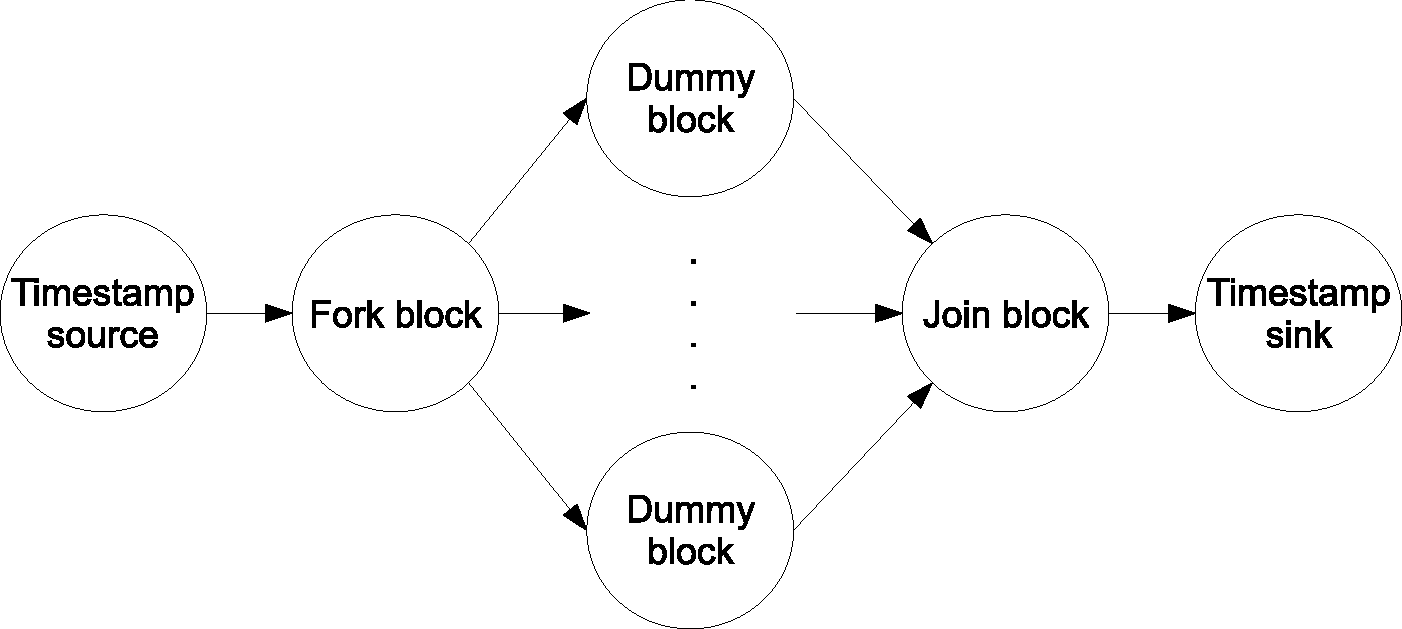
\includegraphics{fig/fig_arch_test_par}}}
%  \newpage
%  \subfloat[]{\label{fig_arch_test_par2}\scalebox{0.27}{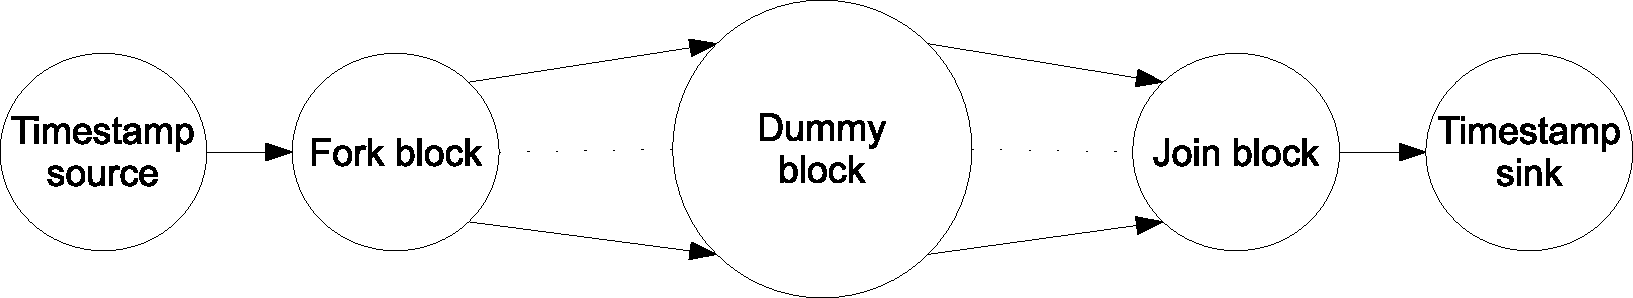
\includegraphics{fig/fig_arch_test_par2}}}
%  \caption{SDRs data flow structures used for the overhead evaluation in terms of the number 
%of blocks in serial (a), the number of data flows in parallel (b), and the number of inputs/outputs (c)}
%  \label{fig_arch_test_all}
%\end{figure}

These structures are composed by three kinds of blocks. The \emph{Timestamp source} block generates samples
which consist of ti\-me\-stamps that represent the time when the sample was generated. The \emph{dummy blocks}
are empty blocks that just propagate their inputs to their outputs. After being generated, the samples will
go through the \emph{dummy block} chain. When a sample arrives at the \emph{Timestamp sink} block, the ti\-me\-stamp
is compared with the current time, obtaining the time the sample took to go through the \emph{dummy block} chain.
Since the \emph{dummy blocks} are empty, this resulting time represents only the overhead imposed by the
architecture on the data flow. There is also the \emph{Fork block} and \emph{Join block} which are used to
fork and join the data flows, respectively.

\subsection{System implementation and configuration}

To evaluate these three structures, we have implemented \hyra on the EPOS operating system running on the 
Xilinx's ML403 Embedded Platform.
The ML403 features a Virtex-4 FPGA with an embedded PowerPC 405 microprocessor. In order to use the same
hardware configuration, we have synthesized the hardware with all of the necessary blocks for all experiments. We
have used the following tools and parameters: ISE/EDK 10.1; GCC 4.0.2; FPGA and microprocessor clocked at 100 MHz;
interconnect structure configured with 32 input/output ports, and 64 FIFOs (8 bit wide with 16 elements); 
the $\alpha$ factor fixed to $1$ in order to provide an evaluation considering low jitter requirements. 

%\tab{table_ml403_sdr_arch_params}{Configuration parameters used on the experiments}

Table \ref{table_ml403_sdr_arch_synt} shows the resource consumption of the generated hardware. Separate
results are shown for \hyra's structures along with the HW dummy blocks, and for the system IPs generated
by EDK (internal memory, memory controller, interruption controller, UART, etc). 
Our architecture alone uses about 65\% of the available logic and 0\% of the available memory. Due to the lack of
memory blocks available on the device, we chose to implement the FIFOs using the SRL16 capabilities to
convert a 4-input LUT into a 16-bit shift register. Howsoever, this apparently high resource
usage is due to the very limited amount of logic available on the used device. When compared to other
system IPs, we can see that \hyra uses slightly more resources then a complete set of basic IO and
memory peripherals.

\tab{table_ml403_sdr_arch_synt}{Amount of HW resources used by the synthesized structures}

%Additionally, the application along with the EPOS operating 
%system compiled for the PowerPC processor resulted in a memory footprint of 47632 bytes of code and 288 bytes of static data.


\subsection{Performance overhead}

We have done tests to determine the performance overhead that we have defined as the latency between the
\emph{Timestamp source and sink} blocks in the three basic data flow structures. We have implemented each
structure in hardware and software and executed tests with the number of dummy blocks ranging from 1 to 16.
In each test $6\times10^7$ samples were generated and we obtained the average value of the latencies of each sample
and the standard deviation which was used to obtain the coefficient of variation. A sampling rate of $1\times10^6$
samples/second was used in the tests with blocks in hardware. For the tests with blocks in software we used a sampling
rate of $1\times10^4$ due to the low speed of the PowerPC processor.

Figures \ref{fig_result_mean_ppc_hw} and \ref{fig_result_coef_ppc_hw} show the results. When using only
software blocks, the overhead grows linearly in relation to the increase in the number of blocks and the number of
inputs and outputs for all structures. The coefficient of variation remained low in all configurations.
When using only HW blocks, the latency was about four orders of magnitude lower than when using
software blocks and, as expected, except for the serial block configuration, the latency remained constant
regardless the size of the structure, due to the full parallelism that can be explored in this kind of
architecture. There is also a null coefficient of variation in the hardware operations.

%\fig{0.4}{fig_result_mean_ppc_hw}{Average latency for blocks in serial, in parallel and with multiple input/output}

%\fig{0.4}{fig_result_coef_ppc_hw}{Coefficient of variation of the proposed architecture latency}

\begin{figure}
  \centering
  \subfloat[Average latency]{\label{fig_result_mean_ppc_hw}\scalebox{0.4}{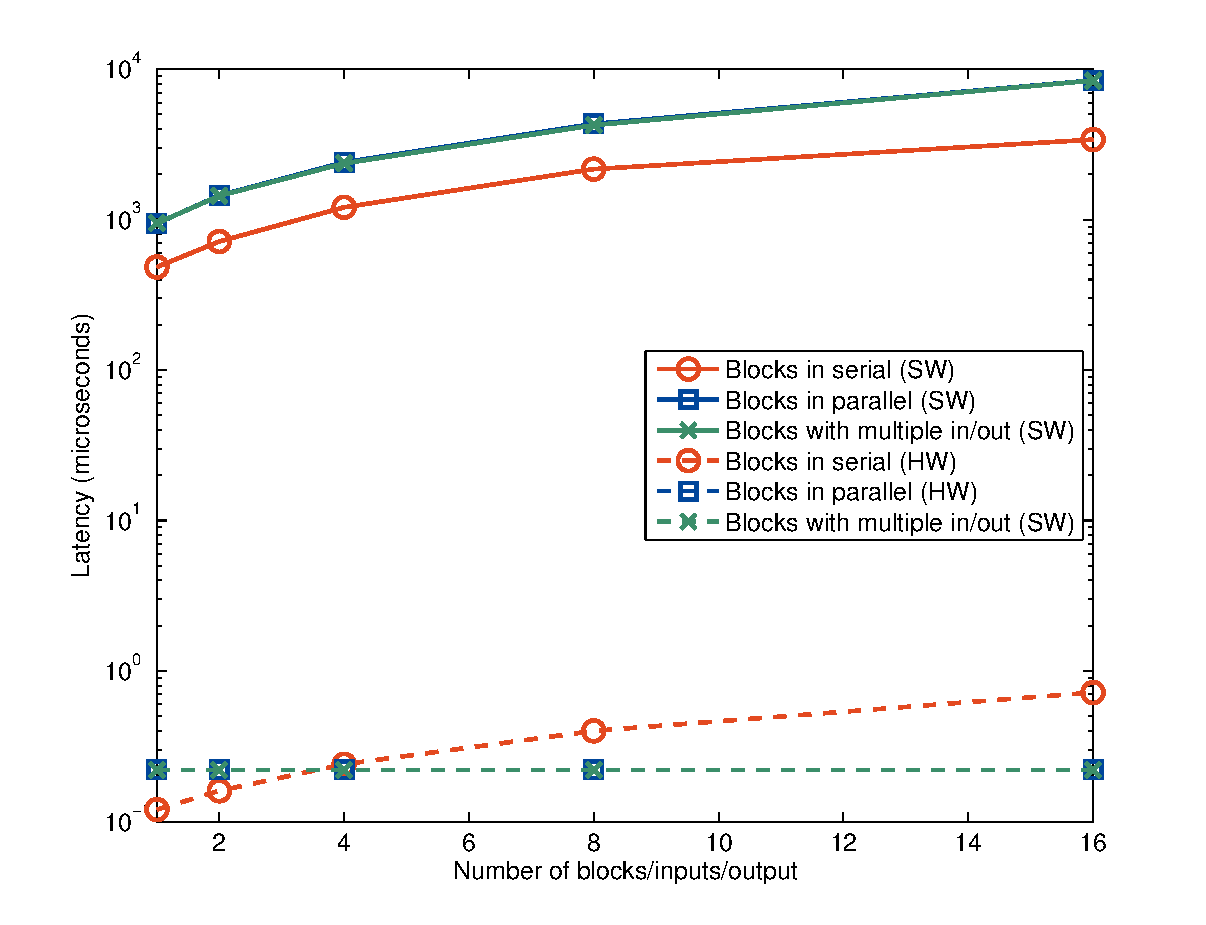
\includegraphics{fig/fig_result_mean_ppc_hw}}} \\
  \subfloat[Coefficient of variation]{\label{fig_result_coef_ppc_hw}\scalebox{0.4}{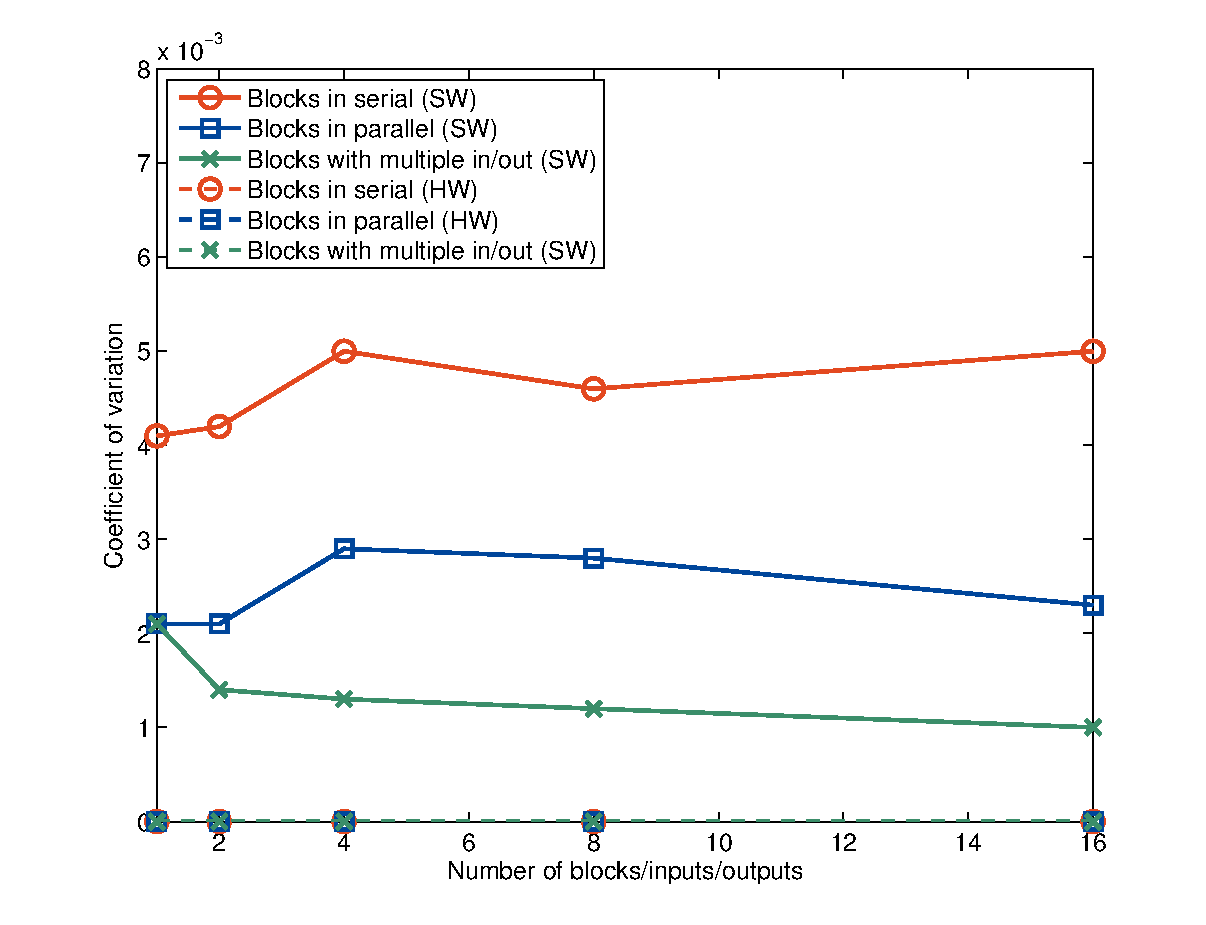
\includegraphics{fig/fig_result_coef_ppc_hw}}}
  \caption{Latency for blocks in serial, in parallel, and with multiple input/output}
  \label{fig_result_ppc_hw}
\end{figure}

%\begin{figure*}[ht]
% \begin{minipage}{0.4\linewidth}
%   \centering
%   \subfloat[Average latency]{\label{fig_result_mean_ppc_hw}\scalebox{0.4}{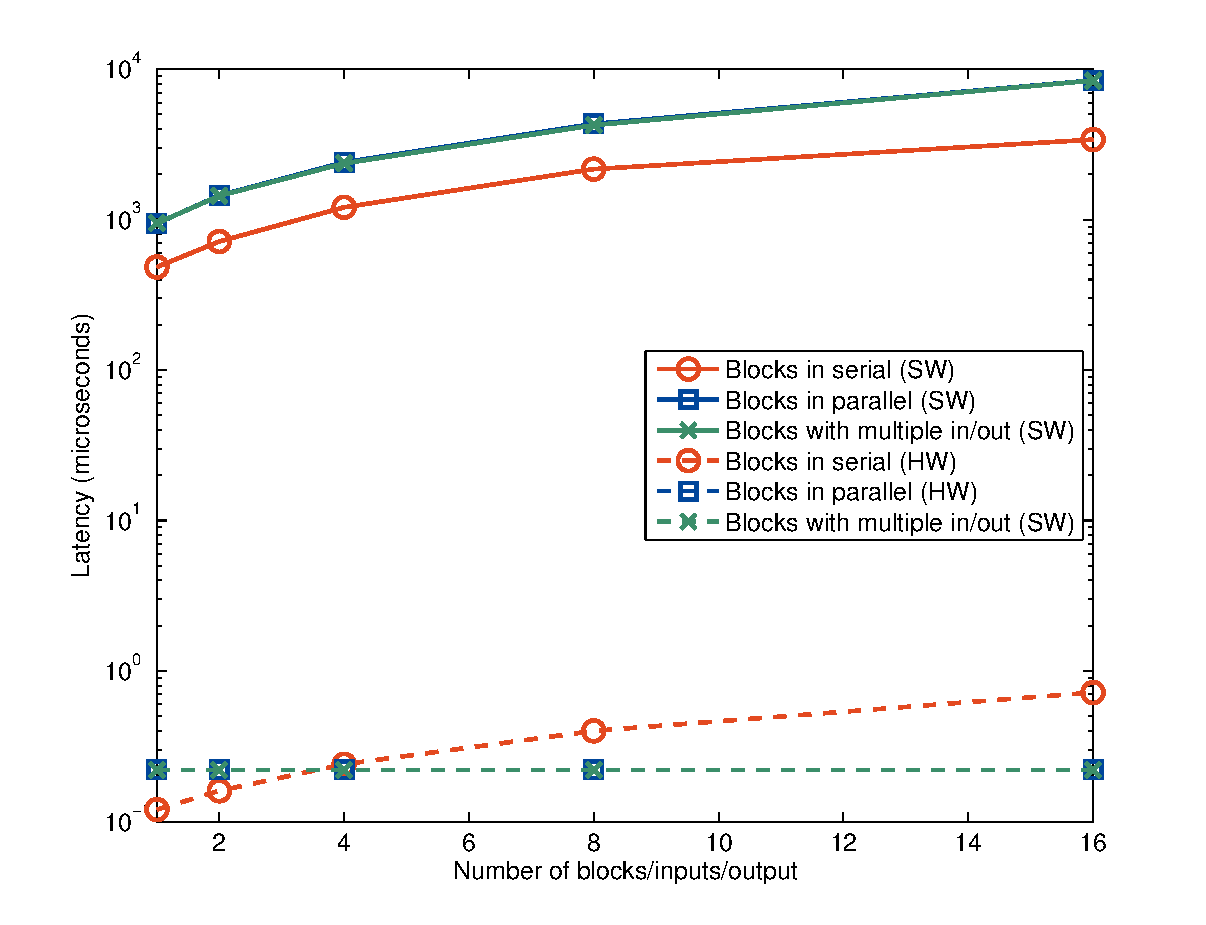
\includegraphics{fig/fig_result_mean_ppc_hw}}} \\
% \end{minipage}
% %\hspace{0.5cm}
%\hspace{0.35\linewidth}
% \begin{minipage}{0.4\linewidth}
%   \centering
%   \subfloat[Coefficient of variation]{\label{fig_result_coef_ppc_hw}\scalebox{0.4}{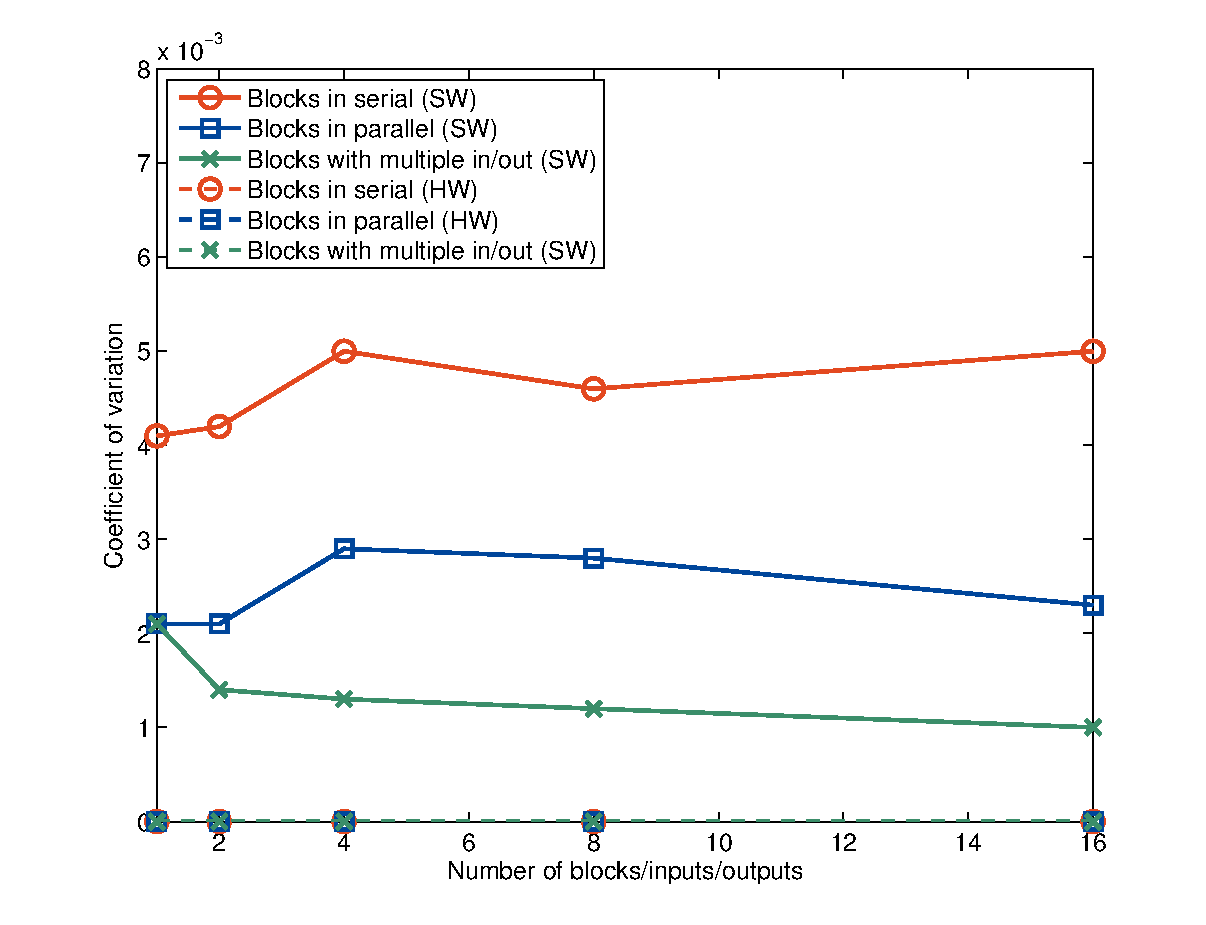
\includegraphics{fig/fig_result_coef_ppc_hw}}}
% \end{minipage}
%\caption{Latency for blocks in serial, in parallel, and with multiple input/output}
%  \label{fig_result_ppc_hw}
%\end{figure*}


%\begin{figure}[ht]
%  \begin{minipage}[htbp]{0.5\linewidth}
%    \centering
%    \scalebox{0.4}{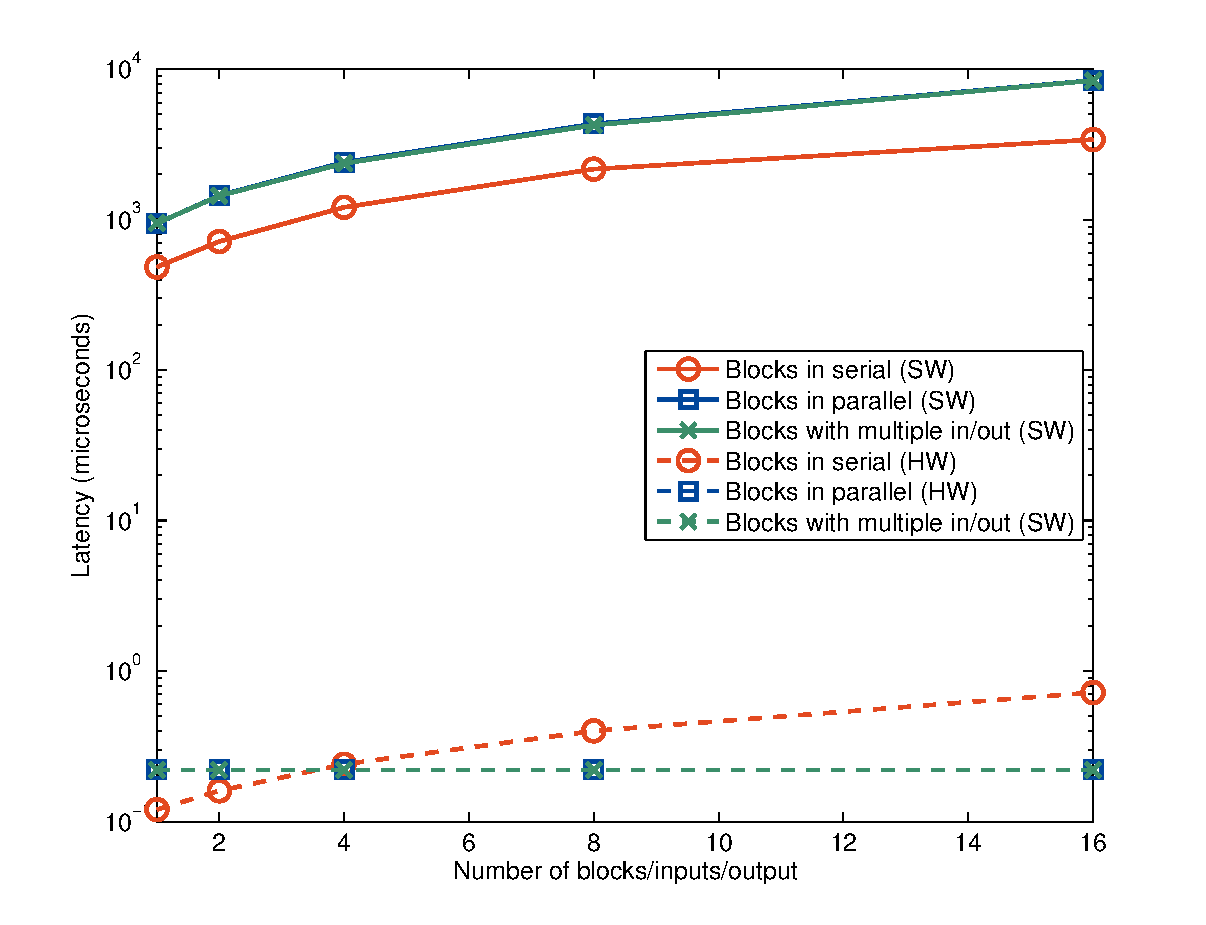
\includegraphics{fig/fig_result_mean_ppc_hw}}
%    \caption{Average latency for blocks in serial, in parallel and with multiple input/output}
%    \label{fig_result_mean_ppc_hw}
%  \end{minipage}
%  \hspace{0.5cm}
%  \begin{minipage}[htbp]{0.5\linewidth}
%    \centering
%    \scalebox{0.4}{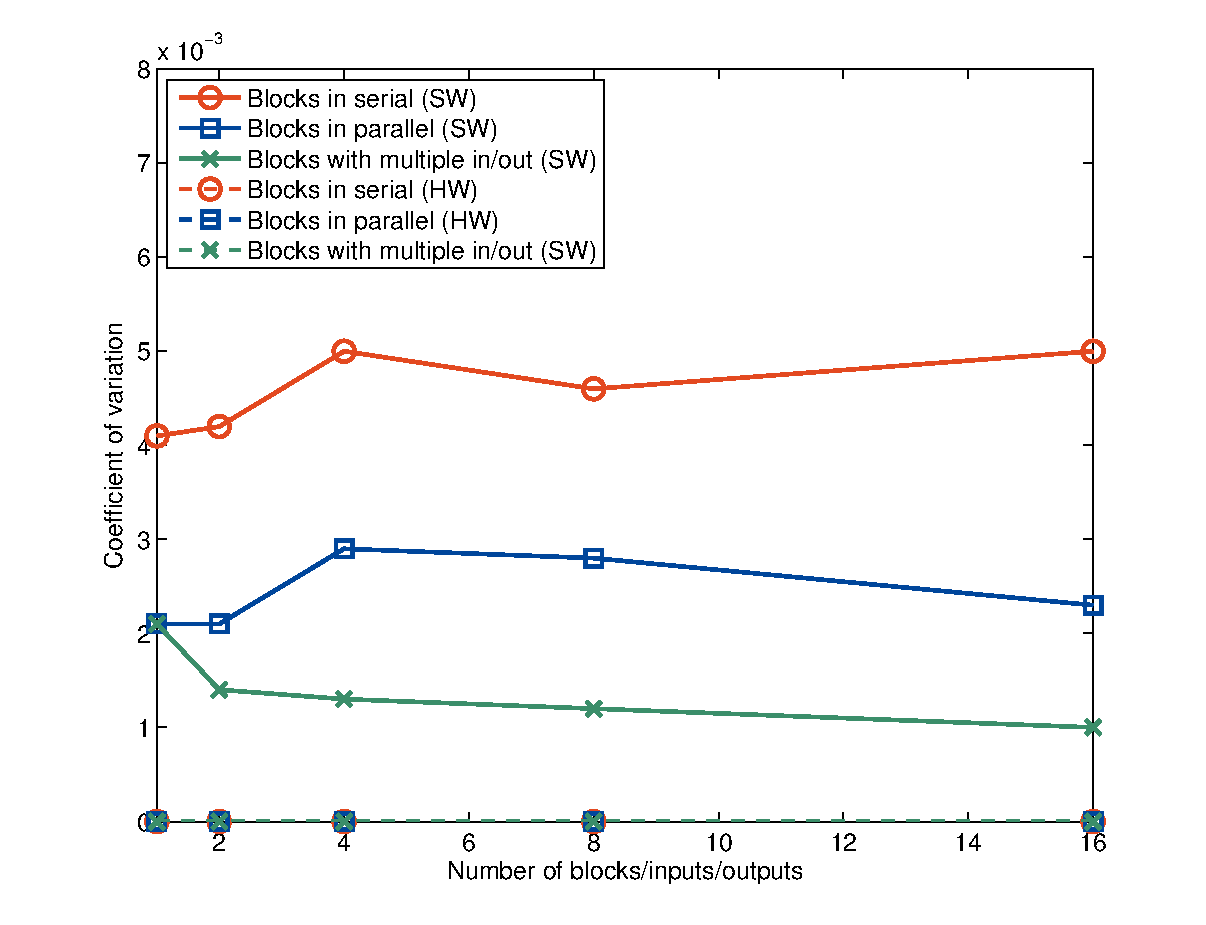
\includegraphics{fig/fig_result_coef_ppc_hw}}
%    \caption{Coefficient of variation of the proposed architecture latency}
%    \label{fig_result_coef_ppc_hw}
%  \end{minipage}
%\end{figure}


To evaluate the communication latency between components implemented in HW and components
implemented in SW, we have used the data flow shown in Figure \ref{fig_result_sw_hw_data_flow} which
cover operations on both \emph{SW-HW FIFOs} and \emph{HW-SW FIFOs}. We have performed the same
experiment described previously on this two structures and verified that the average latency
on both interleaved data flows yielded similar results: $221 \mu s$ and $234 \mu s$ for data flows
\emph{(a)} and \emph{(b)}, respectively. Data flow (a) have more SW blocks then
(b), thus showing a higher SW management overhead. However, both have two \emph{SW-HW FIFOs} and two
\emph{HW-SW FIFOs} connecting the blocks. By comparing the latencies with the ones obtained for SW-only
blocks ($221 \mu s$) and HW-only blocks ($0.31 \mu s$) we can see that the read/write operations SW channels
represents the most significant overhead.

\fig{0.3}{fig_result_sw_hw_data_flow}{Serial data flows with interleaved SW and HW blocks}
%\fig{0.4}{fig_result_sw_hw}{Average latencies on the serial data flow with interleaved SW and HW blocks}
%\tab{table_result_sw_hw}{Average latencies on the serial data flow with interleaved SW and HW blocks}

We also compared the overhead of our architecture to GNU Radio. For this comparison, we replicated the
same tests described previously using GNU Radio running over a Linux operating system in a PC. Our
architecture and EPOS were compiled for the IA32 architecture only with software blocks support, and
evaluated in the same system. For the GNU Radio experiment, we used GNU Radio 3.2.2 running on a Linux
kernel 2.6.28. The result for the serial blocks data flow structure shown in Figure
\ref{fig_result_mean_ia32_gnu} demonstrates that our architecture performance surpasses GNU Radio between
2 and 4 times, and this difference increases as the number of blocks in the processing chain increases.
Figure \ref{fig_result_coef_ia32_gnu} also shows that we are able to achieve smaller latency variations as well.

%\fig[h]{0.4}{fig_result_mean_ia32_gnu}{Average latency of the proposed architecture VS GNU Radio on the serial blocks data flow structure}

%\fig[h]{0.4}{fig_result_coef_ia32_gnu}{Coefficient of variation of the proposed architecture latency VS GNU Radio on the serial blocks data flow structure}

\begin{figure}[t]
  \centering
  \subfloat[Average latency]{\label{fig_result_mean_ia32_gnu}\scalebox{0.4}{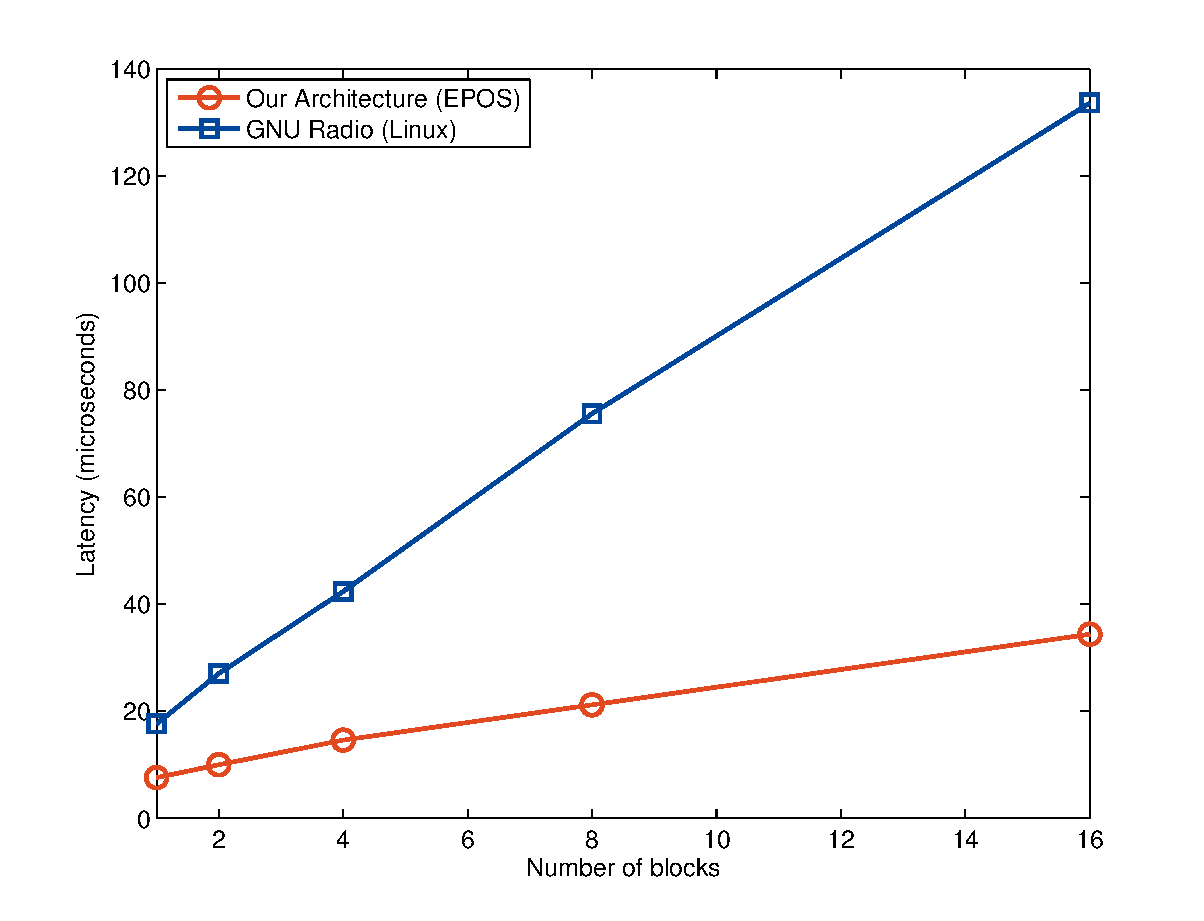
\includegraphics{fig/fig_result_mean_ia32_gnu}}} \\               
  \subfloat[Coefficient of variation]{\label{fig_result_coef_ia32_gnu}\scalebox{0.4}{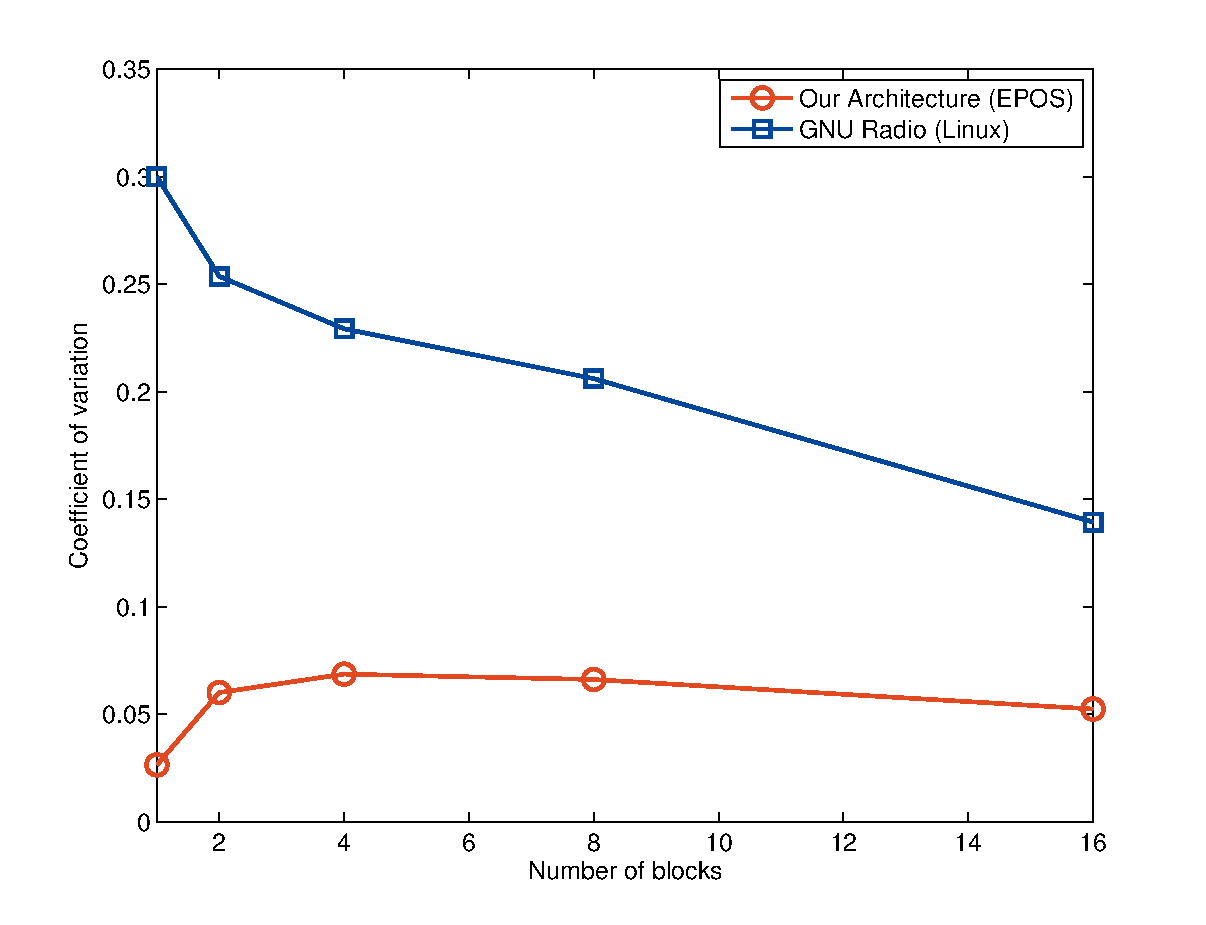
\includegraphics{fig/fig_result_coef_ia32_gnu}}}
  \caption{Latency of the proposed architecture VS GNU Radio on the serial blocks data flow structure}
  \label{fig_result_ia32_gnu}
\end{figure}

%\begin{figure}[ht]
%  \begin{minipage}[htbp]{0.5\linewidth}
%    \centering
%    \scalebox{0.4}{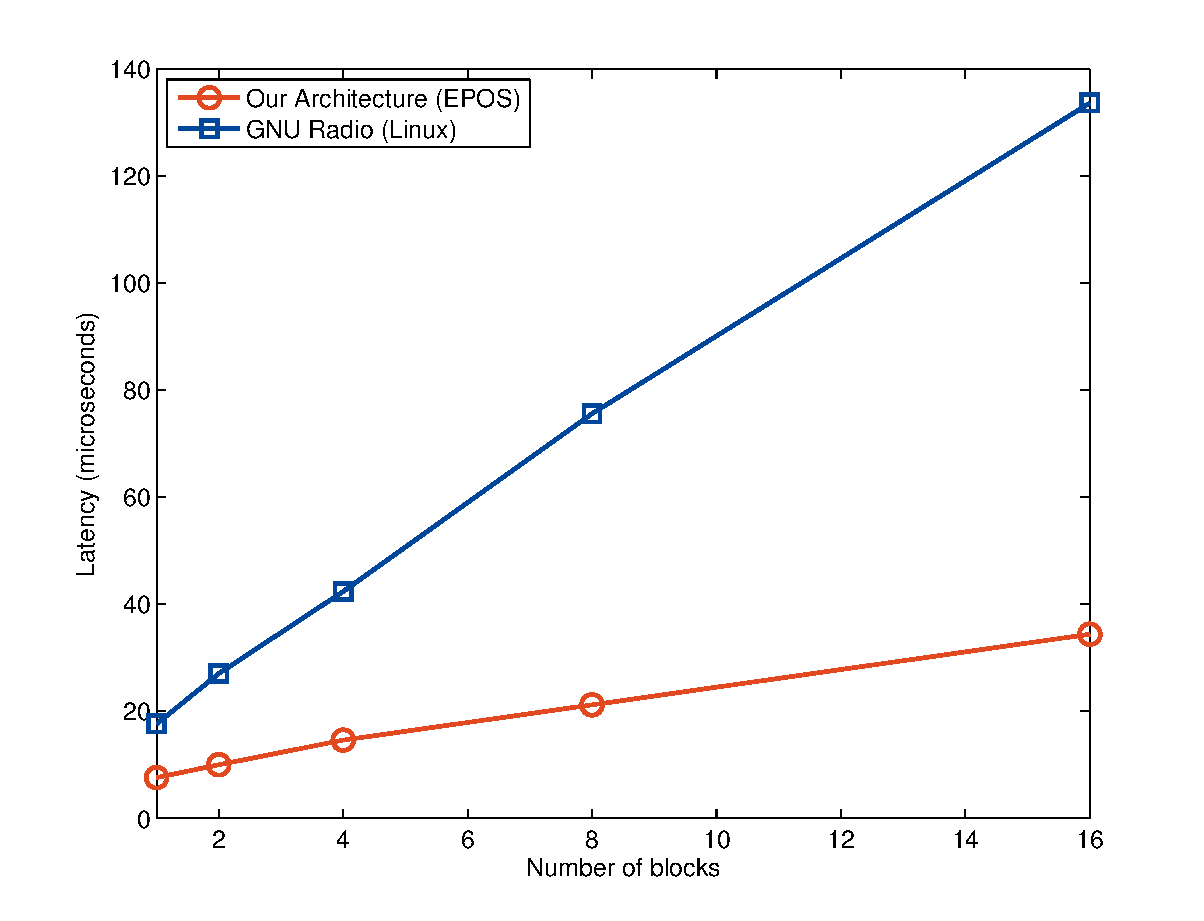
\includegraphics{fig/fig_result_mean_ia32_gnu}}
%    \caption{Average latency of the proposed architecture VS GNU Radio on the serial blocks data flow structure}
%    \label{fig_result_mean_ia32_gnu}
%  \end{minipage}
%  \hspace{0.5cm}
%  \begin{minipage}[htbp]{0.5\linewidth}
%    \centering
%    \scalebox{0.4}{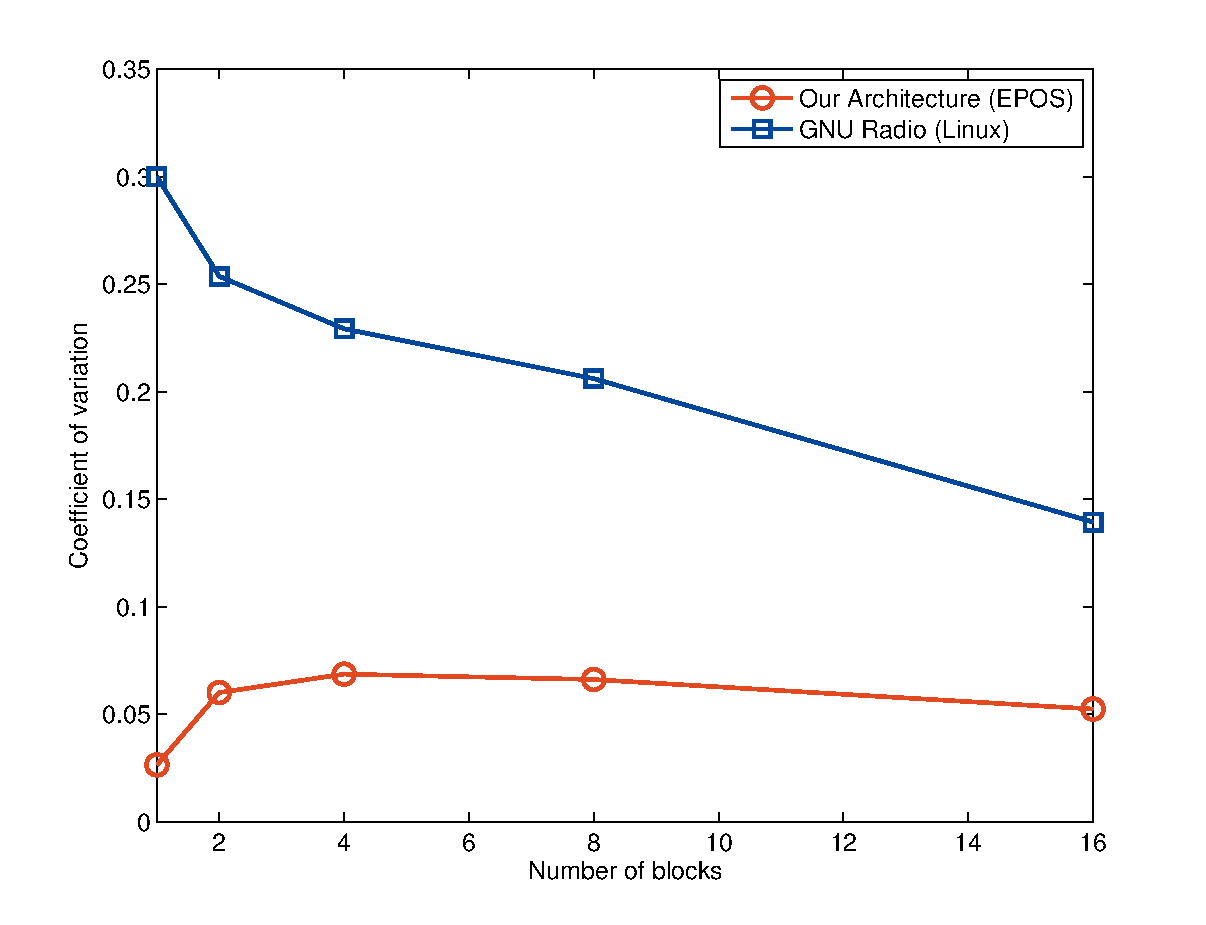
\includegraphics{fig/fig_result_coef_ia32_gnu}}
%    \caption{Coefficient of variation of the proposed architecture latency VS GNU Radio on the serial blocks data flow structure}
%    \label{fig_result_coef_ia32_gnu}
%  \end{minipage}
%\end{figure}


\subsection{Discussion}

The results show that our architecture yields superior performance than an equivalent, in terms of abstraction level,
commonly used architecture. Only software components were used in this comparison, if a hardware device was used
to generate the timestamps, GNU Radio would suffer an additional disadvantage. In GNU Radio, the use of any hardware
device to obtain or sink data from/to the environment requires Linux drivers whose performance is mostly limited by
the kernel's abstraction layer. A previous work~\cite{nychis09} shows that, due to the Linux kernel overhead, the
standard deviation of the time a sample takes to get to the processing chain after being generated in the
RF Front-end is higher than the average time. This problem does not appear in EPOS since the metaprogrammed hardware mediators
are dissolved within the application when the system is compiled, which leads to higher performance. 

However, even with known latency problem, the GNU Radio is widely used and several protocols have been
successfully implemented using it. The results have shown that with our architecture we were able to bring
similar functionality with superior performance to the embedded system domain, which leads to the conclusion
that our architecture is suitable for the implementation of high-end protocols in embedded systems.

%%%%%%%%%%%%%%%%%%%%%%%%%%%%%%%%%%%%%%%%%%%%%%%%%%%%%%%%%%%%%%%%%%%%%%%%%%%%%%
\section{Conclusion}
\label{CONCLUSION}

In this paper we have introduced \hyra, an \emph{Hybrid Radio
 Architecture} that explores the \emph{Hybrid Component} concept within
ADESD to enable the implementation of SDRs as direct mappings of
high-level SDF models. As hybrid components, \hyra\ SDR blocks can be
implemented as arbitrary combination of software and hardware on
FPGA-based platforms. The programmable interconnect infrastructure in
\hyra's framework ensures transparency in this respect.  FIFO channels
can be fine tuned to fulfill the requirements of a given SDR protocol,
while the controller dynamically coordinates the flow of data between
components.

In comparison with other approaches, \hyra\ addresses the implementation
of SDRs in the context of embedded systems from a higher level of
abstraction. Moreover, the evaluation results presented in this paper confirm
that the overhead caused by the proposed architecture in terms of
latency is much smaller than that of GNU Radio, a widely accepted architecture. 
Furthermore, our experiments demonstrated that \hyra\ can be implemented on reconfigurable hardware
platform with minimal additional resources. In combination, this factors
confirm that our architecture meet the requirements for the
implementation of high-end protocols in embedded systems.

\bibliographystyle{IEEEtran}
\bibliography{sdr.bib}

\end{document}



